% Copyright 2018-2020 Melvin Eloy Irizarry-Gelpí
% \setcounter{chapter}{7}
\chapter{Impulse and Momentum}
%
In this experiment, you will study the relationship between impulse and linear momentum.
%
\section{Preliminary}
%
Linear momentum (or just \textbf{momentum}) is a physical quantity that incorporates velocity and mass:
\begin{equation}
    p = m v
\end{equation}
Due to the second law of motion, a net \textbf{force} causes an acceleration (a change in the velocity of an object). This in turn leads to a change in the momentum of an object. The precise relationship between momentum and forces involves a quantity called \textbf{impulse}.

Formally, impulse is defined as the \textbf{area} under the curve in a \textbf{force versus time} graph. In principle, you need calculus to find the area under a curve. In practice you use a simple approximation: you approximate the curve as a \textbf{flat line}. The area under a flat line has the same shape as a rectangle. The area of a rectangle is the length multiplied by the width. Which flat line to use? Since force is in the vertical axis, a flat horizontal line corresponds to a fixed value of force along time. An appropriate choice for the fixed value is the \textbf{time-averaged force} $\bar{F}$. This would correspond to the width of the rectangle. The length of the rectangle is the amount of time $\Delta t$ that the force acts. The ``area'' is thus given by
\begin{equation}
    \text{``Area''} = \bar{F} \times \Delta t = \text{Impulse}
\end{equation}
Impulse has units of force multiplying time. If force is in newtons (N) and time in seconds (s), then impulse has units of N s. However, the newton is equivalent to
\begin{equation}
    1 \ \text{N} = 1 \ \text{kg{ }\textperiodcentered{ }m/s\textsuperscript{2}}
\end{equation}
Thus, the N s is equivalent to
\begin{equation}
    1 \ \text{N{ }\textperiodcentered{ }s} = 1 \ \text{kg{ }\textperiodcentered{ }m/s}
\end{equation}
If you look carefully, these are the same units as momentum. This does not mean that impulse is the same as momentum. Indeed, impulse can also be defined as the \textbf{change in momentum}:
\begin{equation}
    \text{Impulse} = p_{2} - p_{1}
\end{equation}
%
\section{Experiment}
%
In order to verify the relationship between momentum, force, and impulse, you need to use a mechanical system where momentum and force change with time. A cart, moving along a track and colliding with a force sensor is perfect for this. You can consider two kinds of collisions: \textbf{elastic} and \textbf{inelastic} collisions.

In the \textbf{elastic} collisions, you use a spring attachment on the force sensor. When the cart collides with the spring, the spring contracts and then expands, pushing the cart away. The net result is that the cart bounces off the spring. This means that the incoming and outgoing speed of the cart are both non-zero.

In the \textbf{inelastic} collisions, you add some sticky clay on both the force sensor and the cart. When the cart collides with the clay, it sticks to it, and comes to a complete stop. This means that the incoming speed of the cart is non-zero, but the outgoing speed of the cart is zero.

To measure the speed of the cart, you use a photogate placed near the force sensor, in order to measure the speed of the cart just before and just after the collision.

In this way, you collect data on force, and momentum, and the impulse can be determined in two different ways.
%
\section{Analysis}
%
You are going to determine the amount of impulse in two different ways.
%
\subsection{Determine Total Mass of Object}
%
Linear momentum cannot be measured directly. With the speed of the object measured with the photogate, and the mass of the object, you can calculate the experimental value of the linear momentum of the object.

For elastic collisions, the object consist of the cart, the picket fence, and any extra mass added. The total mass is the sum of these three masses.

For inelastic collisions, the object consist of the cart, the picket fence, any extra mass added, and the sticky clay. The total mass is the sum of these four masses.
%
\subsection{Impulse from Change in Momentum}
%
The photogate measures the velocity of the object before the collision ($v_{1}$) and after the collision ($v_{2}$). For an elastic collision, strictly speaking, \textbf{one of the velocities value should be negative} because there is \textbf{a change in the direction} of motion. You have to multiply the value for $v_{1}$ by $-1$ in order to \textbf{make it negative}.

With the values of velocity, and the mass of the object, you can find the momentum of the object \textbf{before} the collision,
\begin{equation}
    p_{1} = m v_{1}
\end{equation}
and the momentum \textbf{after} the collision,
\begin{equation}
    p_{2} = m v_{2}
\end{equation}
The \textbf{change} in momentum is
\begin{equation}
    \Delta p = p_{2} - p_{1}
\end{equation}
This is the first estimate of the amount of impulse during the collision.
%
\subsection{Impulse from Force Acting Over Time}
%
The force sensor measures the amount of \textbf{force on the sensor} during the collision. First you need to determine when the collision is taking place. This involves making a force versus time graph and finding the time $t_{1}$ when the collision begins and the time $t_{2}$ when it ends. With these times you can compute the amount of time that the collision lasts:
\begin{equation}
    \Delta t = t_{2} - t_{1}
\end{equation}
This amount of time is known as the \textbf{duration} of the collision.

When does the collision begin? If the force sensor is zeroed correctly, the force readings should be close to zero before and after the collision. Thus, the collision begins when the force reading change from zero to non-noise non-zero.

You then delete all the force values before and after the collision in the force column. Finally, you can compute the average force during this time period. This gives you the value of $\bar{F}$. Note that $\bar{F}$ is the force on the sensor. What you really want is the amount of force on the cart. You can use Newton's third law of motion and simply change the sign of the force on the sensor to find the force on the cart. With $-\bar{F}$ and $\Delta t$ you can compute the impulse:
\begin{equation}
    \text{impulse} = -\bar{F} \times \Delta t
\end{equation}
This is the second estimate of the amount of impulse during the collision.
%
\section{My Data}
%
There are two experiments: \textbf{elastic} and \textbf{inelastic} collisions. The difference between these experiments is that in the inelastic case, the amount of force during the collision is larger, and the velocity (and also momentum) after the inelastic collision is zero. Besides that, the analysis is almost identical.
%
\subsection{Elastic Collision}
%
In my elastic collision data you will find 12 runs. Here is a breakdown of the amount of extra mass used:
\begin{itemize}
    \item Runs 1, 2, and 3: 0 kg of extra mass
    \item Runs 4, 5, and 6: 0.1 kg of extra mass
    \item Runs 7, 8, and 9: 0.2 kg of extra mass
    \item Runs 10, 11, and 12: 0.3 kg of extra mass
\end{itemize}
You can see the results in Table \ref{table:08.results.elastic}. The third column tabulates the duration of the collision while the force from the spring is acting on the sensor. As you can see, in my case, the duration tends to become larger as the amount of extra mass added to the cart increases. The change in momentum is found in the fourth column. The impulse from the ``area'' formula is found in the fifth column.

In the last column of Table \ref{table:08.results.elastic} you can find a percent difference that quantifies the agreement between the two equivalent definitions of impulse. To calculate the traditional percent difference, you need a (theoretical) expected value and an (experimental) observed value. Here both values for the impulse are determined experimentally, so the percent difference has a modified form. If $I_{1}$ corresponds to the value of impulse determined from the change in momentum, and $I_{2}$ corresponds to the value of impulse determined from the average force and the length of the time interval, then the percent difference is given by
\begin{equation}
    \text{percent difference } = 200 \times \left\vert \frac{I_{1} - I_{2}}{I_{1} + I_{2}} \right\vert
\end{equation}
(The long vertical lines mean taking the absolute value and thus ignoring the sign of the fraction inside).
%
\subsection{Inelastic Collision}
%
In my inelastic collision data you will also find 12 runs. Here is a breakdown of the amount of extra mass used:
\begin{itemize}
    \item Runs 1, 2, and 3: 0 kg of extra mass
    \item Runs 4, 5, and 6: 0.1 kg of extra mass
    \item Runs 7, 8, and 9: 0.2 kg of extra mass
    \item Runs 10, 11, and 12: 0.3 kg of extra mass
\end{itemize}
In the inelastic collisions, both the cart and the force sensor had a sticky clay attachment that enabled the cart to stick to the force sensor during the collision.

The velocity column for each inelastic collision has a single velocity measurement. This value corresponds to $v_{1}$, the velocity of the incoming cart before the collision. The velocity after the inelastic collision is zero.

There is a very important difference between the inelastic collisions and the elastic collisions: In the force versus time graph, after the initial deep well (which is deeper in the inelastic case than in the elastic case), there are peaks and wells that are significant in magnitude and cannot be regarded as noise. For example, the significant region in the force versus time chart for run 1 is in figure \ref{figure.08.run.1}. Beyond this region in time, there are further oscillations, but they are not large enough to be significant and are thus regarded as noise.

You can find my results for the inelastic collisions in Table \ref{table:08.results.inelastic}. Note that the time duration of the collision, in the third column, stays about the same value even though the extra mass is increasing.
%
\section{Your Data}
%
You collected data for elastic collisions. I will make available data for the inelastic collisions. For section V01 the values of the extra mass used are in Table \ref{table:08.inelastic.mass.v01} and in Table \ref{table:08.inelastic.mass.v02} for section V02.

You should have 9 runs for the elastic collisions. You should analyze all of them.

The data files for the inelastic collisions have 12 runs. You should only analyze four runs, chosen as follows:
\begin{itemize}
    \item One run from runs 1, 2, or 3
    \item One run from runs 4, 5, or 6
    \item One run from runs 7, 8, or 9
    \item One run from runs 10, 11, or 12
\end{itemize}
%
% \newpage
% \section{Your Laboratory Report}
% %
% In your lab report you should include:
% \begin{enumerate}
%     \item A table like Table \ref{table:08.results.elastic} with the results for the \textbf{elastic} collisions.
%     \item A table like Table \ref{table:08.results.inelastic} with the results for the \textbf{inelastic} collisions.
%     \item One chart with force in the vertical axis and time in the horizontal axis showing the time region where an \textbf{elastic} collision is happening. See Figure \ref{figure.08.run.1.elastic}.
%     \item One chart with force in the vertical axis and time in the horizontal axis showing the time region where an \textbf{inelastic} collision is happening. See Figure \ref{figure.08.run.1}.
% \end{enumerate}
% You should also answer the following questions:
% \begin{enumerate}
%     \item How does the average force during the elastic collisions compare to the average force during the inelastic collision?
%     \item How does the collision duration $\Delta t$ for the elastic collisions compare to the inelastic collisions?
% \end{enumerate}
%
\newpage
\section{Your Laboratory Worksheet}
%
Please print your work before coming to class.
%
\paragraph{Part 1: Elastic collisions}
%
\begin{enumerate}
    \item Provide one \textbf{line chart} with force in the vertical axis and time in the horizontal axis. Restrict only to the collision time segment. You are free to choose which run to use for the chart.
    \item Provide a \textbf{table} with the mass values for
    \begin{itemize}
        \item the cart;
        \item the picket fence; and
        \item the total mass.
    \end{itemize}
    \item Provide a \textbf{table} with
    \begin{itemize}
        \item the amount of extra mass;
        \item the collision duration $\Delta t$;
        \item the average force $\bar{F}$ during the collision;
        \item the observed impulse $\mathcal{I}$;
        \item the observed change in momentum $\Delta p$; and
        \item the percent difference between the change in momentum and the impulse.
    \end{itemize}
    Include a total of four runs in your table; one run for each distinct extra mass value used.
    \item Are both definitions of impulse consistent?
\end{enumerate}
%
\paragraph{Part 2: Inelastic collisions}
%
\begin{enumerate}
    \item Provide one \textbf{line chart} with force in the vertical axis and time in the horizontal axis. Restrict only to the collision time segment. You are free to choose which run to use for the chart.
    \item Provide a \textbf{table} with the mass values for
    \begin{itemize}
        \item the cart;
        \item the picket fence;
        \item the clay; and
        \item the total mass.
    \end{itemize}
    \newpage
    \item Provide a \textbf{table} with
    \begin{itemize}
        \item the amount of extra mass;
        \item the collision duration $\Delta t$;
        \item the average force $\bar{F}$ during the collision;
        \item the observed impulse $\mathcal{I}$;
        \item the observed change in momentum $\Delta p$; and
        \item the percent difference between the change in momentum and the impulse.
    \end{itemize}
    Include a total of four runs in your table; one run for each distinct extra mass value used.
    \item Are both definitions of impulse consistent?
\end{enumerate}
%
\paragraph{Part 3: Results}
%
\begin{enumerate}
    \item How does the average force during the elastic collisions compare to the average force during the inelastic collision?
    \item How does the collision duration for the elastic collisions compare to the collision duration for the inelastic collisions?
\end{enumerate}
%
\newpage
\section{Table Templates}
%
\begin{table}[ht!]
    \begin{center}
        \begin{tabular}{l | l}
            & \textbf{Mass} (kg) \\
            \hline
            \textbf{Cart} & \\
            \textbf{Picket fence} & \\
            \hline
        \end{tabular}
    \end{center}
    \caption{Sample Table 1}
\end{table}
%
\begin{table}[ht!]
    \begin{center}
        \begin{tabular}{l | l}
            & \textbf{Mass} (kg) \\
            \hline
            \textbf{Cart} & \\
            \textbf{Picket fence} & \\
            \textbf{Clay} & \\
            \hline
        \end{tabular}
    \end{center}
    \caption{Sample Table 2}
\end{table}
%
\begin{table}[ht!]
    \begin{center}
        \begin{tabular}{l | l | l | l | l | l | l}
            \textbf{Run} & \textbf{Extra mass} (kg) & $\Delta t$ (s) & $\bar{F}$ (N) & $\mathcal{I}$ (N s) & $\Delta p$ (kg m/s) & \textbf{P.D.} (\%) \\
            \hline
            1 & & & & & & \\
            2 & & & & & & \\
            3 & & & & & & \\
            \hline
            4 & & & & & & \\
            5 & & & & & & \\
            6 & & & & & & \\
            \hline
            7 & & & & & & \\
            8 & & & & & & \\
            9 & & & & & & \\
            \hline
            10 & & & & & & \\
            11 & & & & & & \\
            12 & & & & & & \\
            \hline
        \end{tabular}
    \end{center}
    \caption{Sample Table 3}
\end{table}
%
\newpage
\section{Example Tables}
%
\begin{table}[ht]
    \centering
    \begin{tabular}{l|r}
        \textbf{Name} & \textbf{Value} (kg) \\
        \hline
        Mass of Cart & 0.5089 \\
        Mass of Fence & 0.0136 \\
        \hline
        Total Mass & 0.5225 \\
        \hline
    \end{tabular}
    \caption{Mass values used during elastic collisions}
    \label{table:08.mass.elastic}
\end{table}
%
\begin{table}[ht]
    \centering
    \begin{tabular}{l|r}
        \textbf{Name} & \textbf{Value} (kg) \\
        \hline
        Mass of Cart & 0.5089 \\
        Mass of Fence & 0.0136 \\
        Mass of Clay & 0.0044 \\
        \hline
        Total Mass & 0.5269 \\
        \hline
    \end{tabular}
    \caption{Mass values used during inelastic collisions}
    \label{table:08.mass.inelastic}
\end{table}
%
\begin{table}[ht]
    \centering
    \begin{tabular}{l|r|r|r|r|r}
        \textbf{Run} & \textbf{Extra Mass} (kg) & $\Delta t$ (s) & $\Delta p$ (kg m/s) & \textbf{Impulse} (N s) & \textbf{P.D.} (\%) \\  
        \hline
        1 & 0 & 0.244 & 0.3725 & 0.3834 & 2.87 \\
        2 & 0 & 0.242 & 0.4504 & 0.4620 & 2.54 \\
        3 & 0 & 0.244 & 0.5392 & 0.5549 & 2.87 \\
        \hline
        4 & 0.1 & 0.268 & 0.6076 & 0.6235 & 2.60 \\
        5 & 0.1 & 0.268 & 0.4712 & 0.4814 & 2.13 \\
        6 & 0.1 & 0.268 & 0.5080 & 0.5211 & 2.55 \\
        \hline
        7 & 0.2 & 0.286 & 0.4480 & 0.4574 & 2.09 \\
        8 & 0.2 & 0.288 & 0.5296 & 0.5422 & 2.36 \\
        9 & 0.2 & 0.284 & 0.4653 & 0.4739 & 1.84 \\
        \hline
        10 & 0.3 & 0.304 & 0.5461 & 0.5550 & 1.61 \\
        11 & 0.3 & 0.302 & 0.5034 & 0.5113 & 1.57 \\
        12 & 0.3 & 0.302 & 0.4688 & 0.4762 & 1.56 \\
        \hline
    \end{tabular}
    \caption{Results for elastic collisions}
    \label{table:08.results.elastic}
\end{table}
%
\begin{table}[ht]
    \centering
    \begin{tabular}{l|r|r|r|r|r}
        \textbf{Run} & \textbf{Extra Mass} (kg) & $\Delta t$ (s) & $\Delta p$ (kg m/s) & \textbf{Impulse} (N s) & \textbf{P.D.} (\%) \\  
        \hline
        1 & 0 & 0.116 & 0.2029 & 0.1981 & 2.39 \\
        2 & 0 & 0.138 & 0.2603 & 0.2624 & 0.82 \\
        3 & 0 & 0.130 & 0.1776 & 0.1732 & 2.49 \\
        \hline
        4 & 0.1 & 0.116 & 0.2470 & 0.2533 & 2.53 \\
        5 & 0.1 & 0.184 & 0.2564 & 0.2677 & 4.32 \\
        6 & 0.1 & 0.174 & 0.2796 & 0.2904 & 3.80 \\
        \hline
        7 & 0.2 & 0.118 & 0.1999 & 0.1871 & 6.59 \\
        8 & 0.2 & 0.096 & 0.1984 & 0.1883 & 5.23 \\
        9 & 0.2 & 0.102 & 0.2195 & 0.2123 & 3.34 \\
        \hline
        10 & 0.3 & 0.136 & 0.3200 & 0.3198 & 0.07 \\
        11 & 0.3 & 0.114 & 0.2390 & 0.2287 & 4.40 \\
        12 & 0.3 & 0.112 & 0.2464 & 0.2373 & 3.76 \\
        \hline
    \end{tabular}
    \caption{Results for inelastic collisions}
    \label{table:08.results.inelastic}
\end{table}
%
\begin{table}[ht]
    \centering
    \begin{tabular}{l|r}
        \textbf{Runs} & \textbf{Extra Mass} (kg) \\
        \hline
        1, 2, and 3 & 0 \\
        4, 5, and 6 & 0.05 \\
        7, 8, and 9 & 0.150 \\
        10, 11, and 12 & 0.250 \\
        \hline
    \end{tabular}
    \caption{Extra mass values used for inelastic collisions for section V01}
    \label{table:08.inelastic.mass.v01}
\end{table}
%
\begin{table}[ht]
    \centering
    \begin{tabular}{l|r}
        \textbf{Runs} & \textbf{Extra Mass} (kg) \\
        \hline
        1, 2, and 3 & 0 \\
        4, 5, and 6 & 0.1 \\
        7, 8, and 9 & 0.150 \\
        10, 11, and 12 & 0.250 \\
        \hline
    \end{tabular}
    \caption{Extra mass values used for inelastic collisions for section V02}
    \label{table:08.inelastic.mass.v02}
\end{table}
%
\newpage
\FloatBarrier
\section{Example Charts}
%
\begin{figure}[ht]
    \centering
    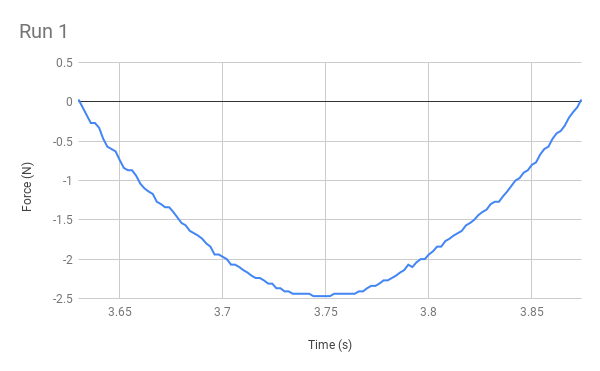
\includegraphics[scale=0.71]{image/08-impulse/Run1-elastic.png}
    \caption{Run 1 for the elastic collisions}
    \label{figure.08.run.1.elastic}
\end{figure}
%
\begin{figure}[ht]
    \centering
    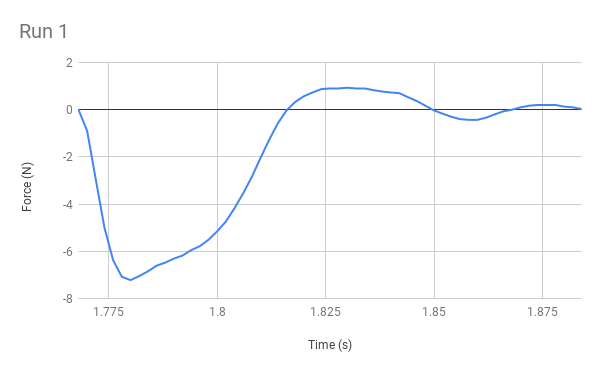
\includegraphics[scale=0.71]{image/08-impulse/Run1-inelastic.png}
    \caption{Run 1 for the inelastic collisions}
    \label{figure.08.run.1}
\end{figure}
%